
\section{Liên trường Nghệ An - Lần 1 NH: 2025--2026}
\vspace{-0.5cm}
\Opensolutionfile{ans}[ans/ans-15-26-2-NgheAn-LienTruong-L1-NLC]
\caulc

\begin{ex}%[2D1N3-2]%[TheHung, Dự án DeTHPT 2025 - 2026]
	Cho hàm số $y=f(x)$ có bảng biến thiên như hình vẽ bên. Mệnh đề nào dưới đây đúng?
	\begin{center}
		
\begin{tikzpicture}
			\tkzTabInit[nocadre=true, lgt=1.2, espcl=2.5]
			{$x$ / 0.8, $y'$ / 0.8, $y$ / 2}
			{$-\infty$, $0$, $1$, $+\infty$}
			\tkzTabLine{ , -, $0$, +, d, -, }
			\tkzTabVar{+/ $+\infty$ , -/ $4$ , +/ $5$ , -/ $-\infty$}
		\end{tikzpicture}
	\end{center}
	\choice
	{$\min\limits_{\mathbb{R}} y = 4$}
	{$y_{CT} = 0$}
	{$\max\limits_{\mathbb{R}} y = 5$}
	{\True $y_{\text{CĐ}} = 5$}
	\loigiai{
		Dựa vào bảng biến thiên, giá trị cực đại của hàm số là $y_{\text{CĐ}} = 5$.
	}
\end{ex}

\begin{ex}%[1D2N2-3]%[TheHung, Dự án DeTHPT 2025 - 2026]
	Tìm công sai $d$ của cấp số cộng $(u_n)$, $n \in \mathbb{N}^*$ có $u_1=1$; $u_4=13$.
	\choice
	{$d=\dfrac{1}{3}$}
	{$d=3$}
	{$d=\dfrac{1}{4}$}
	{\True $d=4$}
	\loigiai{
		Ta có 
		$u_4 = u_1 + 3d \Leftrightarrow d = \dfrac{u_4-u_1}{3}=\dfrac{13-1}{3} = 4$.
	}
\end{ex}

\begin{ex}%[1H8N7-3]%[TheHung, Dự án DeTHPT 2025 - 2026]
	Cho hình chóp $S.ABCD$ có đáy $ABCD$ là hình vuông cạnh $a$. Biết $SA \perp (ABCD)$ và $SA = a\sqrt{3}$. Thể tích của khối chóp $S.ABCD$ là
	\choice
	{$a^3\sqrt{3}$}
	{\True $\dfrac{a^3\sqrt{3}}{3}$}
	{$\dfrac{a^3}{4}$}
	{$\dfrac{a^3\sqrt{3}}{12}$}
	\loigiai{
		\begin{center}
			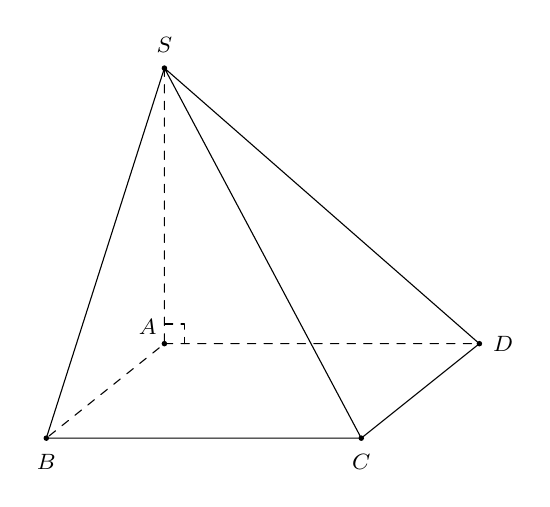
\begin{tikzpicture}[scale=1, font=\footnotesize, line join=round, line cap=round, >=stealth]
				\path
				(0,0) coordinate (A)
				(-1.5,-1.2) coordinate (B)
				(2.5,-1.2) coordinate (C)
				(4,0) coordinate (D)
				(0,3.5) coordinate (S);
				\draw[dashed] (S)--(A)--(B) (A)--(D);
				\draw (S)--(B)--(C)--(D)--cycle (S)--(C);
				\foreach \x/\g in {S/90, A/135, B/-90, C/-90, D/0}
				\fill (\x) circle (1pt) node[shift={(\g:3mm)}]{$\x$};
				% Ký hiệu góc vuông
				\draw[dashed] (A) ++(0,0.25) -- ++(0.25,0) -- ++(0,-0.25);
			\end{tikzpicture}
		\end{center}
		Vì $ABCD$ là hình vuông cạnh $a$ nên $S_{ABCD} = a^2$.\\
		Ta có  $SA \perp (ABCD)$ và $SA = a\sqrt{3}$.\\
		Thể tích của khối chóp $S.ABCD$ là $V = \dfrac{1}{3} \cdot S_{ABCD} \cdot SA = \dfrac{1}{3} \cdot a^2 \cdot a\sqrt{3} = \dfrac{a^3\sqrt{3}}{3}$.
	}
\end{ex}

\begin{ex}%[1D5N1-2]%[TheHung, Dự án DeTHPT 2025 - 2026]
	Một cuộc khảo sát thực hiện để điều tra số giờ sử dụng điện thoại và tivi của $40$ học sinh lớp 11A trong một tuần. Thu được kết quả như sau
	\begin{center}
		\begin{tabular}{|l|c|c|c|c|}
			\hline Thời gian (giờ) &$[0; 2)$ &$[2; 4)$ &$[4; 6)$ &$[6; 8)$ \\
			\hline Số học sinh & $6$ & $18$ & $12$ & $4$ \\
			\hline
		\end{tabular}
	\end{center}
	Nhóm chứa mốt là
	\choice
	{$[4;6)$}
	{$[0;2)$}
	{\True $[2;4)$}
	{$[6;8)$}
	\loigiai{
		Nhóm có tần số lớn nhất là nhóm $[2;4)$ với tần số là $18$.\\
		Do đó, nhóm chứa mốt là nhóm $[2;4)$.
	}
\end{ex}

\begin{ex}%[1D7N2-1]%[TheHung, Dự án DeTHPT 2025 - 2026]
	Đạo hàm của hàm số $y=3^x$ là
	\choice
	{$y' = \dfrac{3^x}{\ln 3}$}
	{$y' = \dfrac{-3^x}{\ln 3}$}
	{$y' = -3^x \ln 3$}
	{\True $y' = 3^x \ln 3$}
	\loigiai{
		Áp dụng công thức đạo hàm $\left(a^x\right)' = a^x \ln a$ (với $a>0, a \ne 1$).\\
		Ta có $y' = \left(3^x\right)' = 3^x \ln 3$.
	}
\end{ex}

\begin{ex}%[1H8N7-1]%[TheHung, Dự án DeTHPT 2025 - 2026]
	Cho lăng trụ tam giác đều $ABC.A'B'C'$ có cạnh đáy $AB = a$, cạnh bên $AA' = 2a$. Khoảng cách giữa hai mặt đáy của lăng trụ bằng
	\choice
	{$a\sqrt{5}$}
	{\True $2a$}
	{$a$}
	{$3a$}
	\loigiai{
		\begin{center}
			\begin{tikzpicture}[scale=1, font=\footnotesize, line join=round, line cap=round, >=stealth]
				\path
				(0,0) coordinate (A)
				(1.5,-1.2) coordinate (B)
				(4,0) coordinate (C)
				($(A)+(0,4)$) coordinate (A')
				($(B)+(0,4)$) coordinate (B')
				($(C)+(0,4)$) coordinate (C');
				\draw (A')--(B')--(C')--cycle;
				\draw (A)--(B)--(C)--(C')--(B') (A')--(A) (B)--(B');
				\draw[dashed] (A)--(C);
				\foreach \x/\g in {A/180, B/-90, C/0, A'/180, B'/0, C'/0}
				\fill (\x) circle (1pt) node[shift={(\g:3mm)}]{$\x$};
			\end{tikzpicture}
		\end{center}
		Vì $ABC.A'B'C'$ là lăng trụ tam giác đều nên lăng trụ này là lăng trụ đứng.\\
		Do đó, khoảng cách giữa hai mặt đáy của lăng trụ chính là độ dài cạnh bên $AA' = 2a$.
	}
\end{ex}


\begin{ex}%[1D1H5-3]%[TheHung, Dự án DeTHPT 2025 - 2026]
	Phương trình $\sin x = -\dfrac{\sqrt{3}}{2}$ có tổng nghiệm dương nhỏ nhất và nghiệm âm lớn nhất bằng
	\choice
	{$2\pi$}
	{$\dfrac{\pi}{3}$}
	{$\dfrac{4\pi}{3}$}
	{\True $\pi$}
	\loigiai{
		Ta có $\sin x = -\dfrac{\sqrt{3}}{2} = \sin\left(-\dfrac{\pi}{3}\right) \Leftrightarrow \left[\begin{aligned} &x = -\dfrac{\pi}{3} + k2\pi \\ &x = \dfrac{4\pi}{3} + k2\pi \end{aligned}\right. (k \in \mathbb{Z})$.\\
		Nghiệm dương nhỏ nhất của phương trình là $x = \dfrac{4\pi}{3}$ (ứng với họ nghiệm thứ hai khi $k=0$).\\
		Nghiệm âm lớn nhất của phương trình là $x = -\dfrac{\pi}{3}$ (ứng với họ nghiệm thứ nhất khi $k=0$).\\
		Do đó, tổng nghiệm dương nhỏ nhất và nghiệm âm lớn nhất của phương trình là $$\dfrac{4\pi}{3} + \left(-\dfrac{\pi}{3}\right) = \pi.$$
	}
\end{ex}

\begin{ex}%[2D1N4-1]%[TheHung, Dự án DeTHPT 2025 - 2026]
	Tiệm cận đứng của đồ thị hàm số $y = \dfrac{5}{x-1}$ là đường thẳng có phương trình
	\choice
	{$x=5$}
	{$y=0$}
	{$y=1$}
	{\True $x=1$}
	\loigiai{
		Ta có $\left\{\begin{aligned}&\lim\limits_{x \to 1^-} y = -\infty \\ &\lim\limits_{x \to 1^+} y = +\infty\end{aligned}\right. \Rightarrow x=1$ là đường tiệm cận đứng của đồ thị hàm số.
	}
\end{ex}

\begin{ex}%[2D1N5-4]
	Số giao điểm của đồ thị hai hàm số $y = x^2 - 3x - 1$ và $y = x^3 - 1$ là
	\choice
	{\True $1$}
	{$0$}
	{$3$}
	{$2$}
	\loigiai{
		Phương trình hoành độ giao điểm của hai đồ thị
		\[x^3 - 1 = x^2 - 3x - 1 \Leftrightarrow x^3 - x^2 + 3x = 0 \Leftrightarrow x(x^2 - x + 3) = 0 \Leftrightarrow x = 0.\]		
		Vậy đồ thị hai hàm số có $1$ giao điểm.
	}
\end{ex}

\begin{ex}%[1H8N7-1]%[TheHung, Dự án DeTHPT 2025 - 2026]
	\immini{Cho hình lập phương $ABCD.A'B'C'D'$. Hãy chọn kết luận sai.
		\choice
		{$A'B \parallel (CDD'C')$}
		{$CC' \parallel (ABB'A')$}
		{\True $BD \parallel A'C'$}
		{$(ABCD) \parallel (A'B'C'D')$}}{\begin{tikzpicture}[scale=0.5, font=\footnotesize, line join=round, line cap=round, >=stealth]
			\path
			(0,0) coordinate (B')
			(2.5,0) coordinate (C')
			(3.5,1.2) coordinate (D')
			(1,1.2) coordinate (A')
			($(B')+(0,2.5)$) coordinate (B)
			($(C')+(0,2.5)$) coordinate (C)
			($(D')+(0,2.5)$) coordinate (D)
			($(A')+(0,2.5)$) coordinate (A);
			\draw (B')--(C')--(D') (B)--(C)--(D)--(A)--cycle (B)--(B') (C)--(C') (D)--(D');
			\draw[dashed] (A')--(B') (A')--(D') (A')--(A);
			\foreach \x/\g in {A/135, B/180, C/0, D/0, A'/180, B'/180, C'/0, D'/0}
			{
				\fill[red!80!black] (\x) circle (1.5pt);
				\node[shift={(\g:3mm)}] at (\x) {$\x$};
			}
	\end{tikzpicture}}
	
	\loigiai{
		Ta có $BD\parallel B'D'$ mà $B'D'$ và $A'C'$ là hai đường chéo của hình bình hành $A'B'C'D'$ nên $BD \parallel A'C'$ là phương án sai.		
	}
\end{ex}

\begin{ex}%[2D1N1-2]%[TheHung, Dự án DeTHPT 2025 - 2026]
	Cho hàm số $y=f(x)$ xác định và liên tục trên khoảng $(-\infty;+\infty)$, có bảng biến thiên như hình sau
	\begin{center}
		
\begin{tikzpicture}
			\tkzTabInit[nocadre=true, lgt=1.2, espcl=2.5]
			{$x$ / 0.8, $y'$ / 0.8, $y$ / 2}
			{$-\infty$, $-1$, $1$, $+\infty$}
			\tkzTabLine{ , +, $0$, -, $0$, +, }
			\tkzTabVar{-/ $-\infty$ , +/ $2$ , -/ $-1$ , +/ $+\infty$}
		\end{tikzpicture}
	\end{center}
	Mệnh đề nào sau đây đúng?
	\choice
	{Hàm số nghịch biến trên khoảng $(-\infty;-1)$}
	{Hàm số nghịch biến trên khoảng $(-\infty;2)$}
	{\True Hàm số đồng biến trên khoảng $(1;+\infty)$}
	{Hàm số đồng biến trên khoảng $(-1;+\infty)$}
	\loigiai{
		Dựa vào bảng biến thiên, ta có hàm số đồng biến trên các khoảng $(-\infty;-1)$ và $(1;+\infty)$.
	}
\end{ex}

\begin{ex}%[2D1N5-1]%[TheHung, Dự án DeTHPT 2025 - 2026]
	\immini{Đường cong trong hình dưới là đồ thị của hàm số nào?
		\choice
		{$y = -x^3 + 3x^2 - 4$}
		{\True $y = -x^3 + 3x^2 + 1$}
		{$y = x^3 - 3x^2 + 1$}
		{$y = -x^3 + 2x^2 - 1$}}{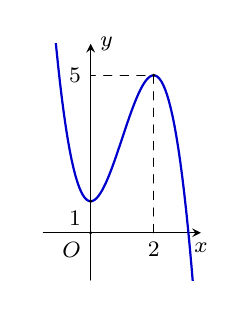
\begin{tikzpicture}[scale=0.4, font=\footnotesize, line join=round, line cap=round, >=stealth]
			% Vẽ trục tọa độ
			\draw[->] (-1.5,0) -- (3.5,0) node[below] {$x$};
			\draw[->] (0,-1.5) -- (0,6) node[right] {$y$};
			\fill (0,0) circle (1.5pt) node[below left] {$O$};			
			
			\clip (-2,-1.5) rectangle (4,6);			\draw[thick, blue!80!black, samples=100, domain=-2:4] plot (\x, {-\x*\x*\x + 3*\x*\x + 1});			
			
			\draw[dashed] (2,0) node[below] {$2$} -- (2,5) -- (0,5) node[left] {$5$};
			\fill (2,5) circle (1.5pt);
			\fill (0,1) circle (1.5pt) node[below left] {$1$};
	\end{tikzpicture}}
	
	\loigiai{
		Đồ thị hàm số đã cho có dạng hàm số bậc ba $y = ax^3 + bx^2 + cx + d$ với $a<0$ và đi qua điểm $(0;1)$ nên phương án thỏa là $y = -x^3 + 3x^2 + 1$.
	}
\end{ex}

\Closesolutionfile{ans}

\cauds
\Opensolutionfile{ans}[ans/ans-15-26-2-NgheAn-LienTruong-L1-DS]

\begin{ex}%[1D6H4-6]%[TheHung, Dự án DeTHPT 2025 - 2026]
	Mức cường độ âm $L$ ($\mathrm{dB}$) được tính bởi công thức $L=10\log\dfrac{I}{10^{-12}}$, trong đó $I$ $\left(\mathrm{W}/\mathrm{m}^2\right)$ là cường độ âm. Để đảm bảo sức khỏe cho công nhân, mức cường độ âm trong một nhà máy phải giữ sao cho không vượt quá $85\mathrm{dB}$. %Xét tính đúng sai của các khẳng định sau:
	\choiceTF
	{\True $L=10\log I + 120$}
	{Nếu cường độ âm $I=1000$ $\left(\mathrm{W}/\mathrm{m}^2\right)$ thì mức cường độ âm không vượt quá $125\mathrm{dB}$}
	{\True Để mức cường độ âm không vượt quá $130\mathrm{dB}$ thì cần cường độ âm $I \le 10$ $\left(\mathrm{W}/\mathrm{m}^2\right)$}
	{\True Cường độ âm của nhà máy đó không vượt quá $10^{-3{,}5}$ $\left(\mathrm{W}/\mathrm{m}^2\right)$ thì đảm bảo sức khỏe cho công nhân}
	\loigiai{
		
		\begin{itemchoice}
			\itemch Ta có 
			$L = 10\log \dfrac{I}{10^{-12}} = 10\left(\log I - \log 10^{-12}\right) = 10\log I + 120$.
			
			\itemch Thay $I = 1000 = 10^3\left(\mathrm{W}/\mathrm{m}^2\right)$ vào công thức, ta được
			$$L = 10\log 10^3 + 120 = 10\cdot 3 + 120 = 150\ (\mathrm{dB}).$$	
			
			\itemch Điều kiện để mức cường độ âm không vượt quá $130\mathrm{dB}$ là $L \le 130$. Khi đó
			$$10\log I + 120 \le 130 \Leftrightarrow 10\log I \le 10 \Leftrightarrow \log I \le 1 \Leftrightarrow I \le 10\ \left(\mathrm{W}/\mathrm{m}^2\right).$$			
			\itemch Để đảm bảo sức khỏe, mức cường độ âm phải không vượt quá $85\mathrm{dB}$, tức là $L \le 85$. Khi đó
			$$10\log I + 120 \le 85 \Leftrightarrow 10\log I \le -35 \Leftrightarrow \log I \le -3{,}5 \Leftrightarrow I \le 10^{-3{,}5}\ \left(\mathrm{W}/\mathrm{m}^2\right).$$		
		\end{itemchoice}
	}
\end{ex}

\begin{ex}%[2D1H3-1]%[TheHung, Dự án DeTHPT 2025 - 2026]
	Cho hàm số $y = f(x) = ax^3 + bx^2 + cx + d$ có bảng biến thiên như sau:
	\begin{center}
		
\begin{tikzpicture}
			\tkzTabInit[nocadre=false,lgt=1.2,espcl=2.5]{$x$ / .7, $y'$ / .7, $y$ / 2}{$-\infty$, $1$, $3$, $+\infty$}
			\tkzTabLine{ , -, $0$, +, $0$, -,  }
			\tkzTabVar{+/$+\infty$, -/$2$, +/$4$, -/$-\infty$}
		\end{tikzpicture}
	\end{center}
	\choiceTF
	{\True Hàm số có hệ số $a < 0$}
	{\True Đồ thị hàm số đi qua hai điểm $(1; 2)$, $(3; 4)$}
	{$f'(x)=0$ tại các giá trị $x = 2$, $x = 4$}
	{Giá trị nhỏ nhất của hàm số trên $[2; 4]$ bằng $\dfrac{7}{2}$}
	\loigiai{
		\begin{itemchoice}
			\itemch Từ bảng biến thiên, ta có $\lim\limits_{x \to +\infty} f(x) = -\infty \Rightarrow$ hệ số $a < 0$. 			
			\itemch Đồ thị hàm số có hai điểm cực trị $(1; 2)$ và $(3; 4)$.
			
			\itemch Từ bảng biến thiên, ta thấy $f'(x) = 0 \Leftrightarrow \hoac{&x=1 \\ &x=3.}$ 
			
			\itemch Ta có $y' = f'(x) = 3ax^2 + 2bx + c$.
			Vì đồ thị hàm số có hai điểm cực trị $A(1; 2)$ và $B(3; 4)$ nên ta có hệ:
			$$ \heva{&f'(1) = 0 \\ &f(1) = 2 \\ &f'(3) = 0 \\ &f(3) = 4} \Leftrightarrow \heva{&3a + 2b + c = 0 \\ &a + b + c + d = 2 \\ &27a + 6b + c = 0 \\ &27a + 9b + 3c + d = 4} \Leftrightarrow \heva{&a = -\dfrac{1}{2} \\ &b = 3 \\ &c = -\dfrac{9}{2} \\ &d = 4.} $$
			Suy ra hàm số là $f(x) = -\dfrac{1}{2}x^3 + 3x^2 - \dfrac{9}{2}x + 4$.
			
			Ta xét trên đoạn $[2; 4]$, có $f(2) = 3$, $f(3) = 4$, $f(4) = 2$.
			Do đó $\min\limits_{[2; 4]} f(x) = 2 \neq \dfrac{7}{2}$. 
		\end{itemchoice}
	}
\end{ex}

\begin{ex}%[2D1V3-6]%[TheHung, Dự án DeTHPT 2025 - 2026]
	\immini{Từ một tấm bìa mỏng hình lục giác đều $ABCDEF$ cạnh $4$ cm, bên trong có một lục giác đều nhỏ hơn. Các đường chéo $AD$, $BE$, $CF$ cắt nhau tại $O$, cắt cạnh lục giác đều nhỏ tại $M$ (như hình vẽ). Đặt $OM = x$ (cm). Bạn Khôi cắt bỏ $6$ tam giác cân bằng nhau có cạnh đáy là cạnh của lục giác đều ban đầu và đỉnh là đỉnh của lục giác đều nhỏ phía trong rồi gấp lên sao cho các đỉnh $A$, $B$, $C$, $D$, $E$, $F$ trùng nhau tạo thành một khối chóp lục giác đều.}{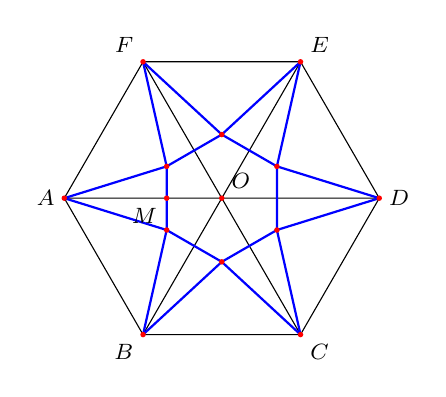
\begin{tikzpicture}[font=\footnotesize, line join=round, line cap=round, scale=0.5]
			\def\R{4}
			\def\x{1.4}
			\def\r{\x*2*sqrt(3)/3} 
			
			%
			\coordinate (A) at (-\R, 0);
			\coordinate (B) at ({-\R*cos(60)}, {-\R*sin(60)});
			\coordinate (C) at ({\R*cos(60)}, {-\R*sin(60)});
			\coordinate (D) at (\R, 0);
			\coordinate (E) at ({\R*cos(60)}, {\R*sin(60)});
			\coordinate (F) at ({-\R*cos(60)}, {\R*sin(60)});
			\coordinate (O) at (0, 0);
			
			
			\coordinate (V6) at (-\x, {\x*sqrt(3)/3});
			\coordinate (V1) at (-\x, {-\x*sqrt(3)/3});
			\coordinate (V2) at (0, {-\r});
			\coordinate (V3) at (\x, {-\x*sqrt(3)/3});
			\coordinate (V4) at (\x, {\x*sqrt(3)/3});
			\coordinate (V5) at (0, {\r});			
			\coordinate (M) at (-\x, 0);			
			\draw[thin] (A) -- (D) (B) -- (E) (C) -- (F) (A)--(B)--(C)--(D)--(E)--(F)--(A);			
			
			\draw[thick, blue] (V1) -- (V2) -- (V3) -- (V4) -- (V5) -- (V6) -- cycle;			
			\draw[thick, blue] (A) -- (V6) (A) -- (V1)
			(B) -- (V1) (B) -- (V2)
			(C) -- (V2) (C) -- (V3)
			(D) -- (V3) (D) -- (V4)
			(E) -- (V4) (E) -- (V5)
			(F) -- (V5) (F) -- (V6);			
			
			\node[left] at (A) {$A$};
			\node[below left] at (B) {$B$};
			\node[below right] at (C) {$C$};
			\node[right] at (D) {$D$};
			\node[above right] at (E) {$E$};
			\node[above left] at (F) {$F$};
			\node[above right] at (O) {$O$};
			\node[below left] at (M) {$M$};
			
			
			\foreach \p in {A,B,C,D,E,F,V1,V2,V3,V4,V5,V6,O,M} {
				\fill[red] (\p) circle (2pt);
			}
	\end{tikzpicture}}
	
	\choiceTF
	{\True Tam giác $OAB$ đều có cạnh bằng $4$ cm}
	{Cạnh đáy của khối chóp lục giác đều bằng $\dfrac{x\sqrt{3}}{6}$ (cm)}
	{\True Đường cao của khối chóp lục giác đều bằng $\sqrt{16-8x}$ (cm)}
	{Thể tích lớn nhất của khối chóp lục giác đều có thể đạt được là $\dfrac{256\sqrt{10}}{375}$ ($\text{cm}^3$)}
	\loigiai{
		\begin{itemchoice}
			\itemch Tam giác $OAB$ là tam giác đều có cạnh bằng cạnh của lục giác đều nên $OA=OB=AB=4$ cm. 
			
			\itemch Khối chóp lục giác đều khi gấp lên sẽ nhận lục giác nhỏ bên trong làm mặt đáy. Khoảng cách từ tâm $O$ đến cạnh của lục giác nhỏ chính là $OM = x$. \\
			Vì $OM$ là độ dài đường cao của tam giác đều cấu tạo nên đáy do đó cạnh đáy của khối chóp lục giác đều bằng $\dfrac{2}{\sqrt{3}}x = \dfrac{2\sqrt{3}}{3}x$. 
			
			\itemch Khi gấp lên, các điểm $A, B, C, \dots$ chập lại thành đỉnh chóp.\\
			 Đoạn $AM$ trở thành đường sinh của mặt bên (với hình chiếu là $OM$).\\ Ta có $AM = OA - OM = 4 - x$. \\
			
			Suy ra chiều cao khối chóp lục giác đều là $\sqrt{AM^2 - OM^2} = \sqrt{(4-x)^2 - x^2} = \sqrt{16-8x}$. 
			
			\itemch Diện tích đáy của khối chóp là $6 \cdot \dfrac{\sqrt{3}}{4} \left(\dfrac{2\sqrt{3}}{3}x\right)^2 = 2\sqrt{3}x^2$. \\
			Thể tích khối chóp lục giác đều là 
			$$V = \dfrac{1}{3} \cdot \sqrt{16-8x} \cdot 2\sqrt{3}x^2 = \dfrac{2\sqrt{3}}{3} \sqrt{16x^4 - 8x^5}.$$
			Xét hàm số $f(x) = 16x^4 - 8x^5$ với $x \in (0; 2)$.\\
			Ta có $f'(x) = 64x^3 - 40x^4$.\\ Cho $f'(x) = 0 \Leftrightarrow x^3(64 - 40x) = 0 \Rightarrow x = \dfrac{8}{5}$.\\
			Do đó $V$ đạt giá trị lớn nhất tại $x = \dfrac{8}{5}$.\\
		 Thể tích lớn nhất của khối chóp lục giác đều bằng $\dfrac{2\sqrt{3}}{3} \sqrt{16\left(\dfrac{8}{5}\right)^4 - 8\left(\dfrac{8}{5}\right)^5} = \dfrac{512\sqrt{15}}{375}$. 
		\end{itemchoice}
	}
\end{ex}

\begin{ex}%[0D0V2-3]%[TheHung, Dự án DeTHPT 2025 - 2026]
	An và Bình rủ nhau đi câu cá vào ngày nghỉ cuối tuần. Xác suất câu được cá của An là $0{,}6$. Xác suất câu được cá của Bình là $0{,}3$. Khi đó ta có:
	\choiceTF
	{\True Xác suất An không câu được cá bằng $0{,}4$}
	{Xác suất có đúng $1$ người câu được cá bằng $0{,}34$}
	{Xác suất để cả $2$ người đều không câu được cá bằng $0{,}3$}
	{\True Xác suất có ít nhất $1$ người câu được cá bằng $0{,}72$}
	\loigiai{
		Gọi $A$ là biến cố \lq\lq An câu được cá\rq\rq và $B$ là biến cố \lq\lq Bình câu được cá \rq\rq.\\
		Suy ra $\overline{A}$ là biến cố \lq\lq An không câu được cá\rq\rq và $\overline{B}$ là biến cố \lq\lq Bình không câu được cá\rq\rq.\\
		Theo giả thiết $\mathrm{P}(A)=0{,}6 \Rightarrow \mathrm{P}\left(\overline{A}\right)=1-0{,}6=0{,}4$; $\mathrm{P}(B)=0{,}3 \Rightarrow \mathrm{P}\left(\overline{B}\right)=1-0{,}3=0{,}7$.
		\begin{itemchoice}
			\itemch Ta có xác suất An không câu được cá là $\mathrm{P}\left(\overline{A}\right)=0{,}4$. 
			
			\itemch Biến cố \lq\lq Có đúng $1$ người câu được cá\rq\rq là $A\overline{B} \cup \overline{A}B$.\\
			Vì việc An và Bình câu được cá là hai hành động độc lập nên $A, B$ là hai biến cố độc lập. Do đó
			$$ \mathrm{P}\left(A\overline{B} \cup \overline{A}B\right) = \mathrm{P}\left(A\overline{B}\right) + \mathrm{P}\left(\overline{A}B\right) = \mathrm{P}(A)\cdot\mathrm{P}\left(\overline{B}\right) + \mathrm{P}\left(\overline{A}\right)\cdot\mathrm{P}(B) = 0{,}6 \cdot 0{,}7 + 0{,}4 \cdot 0{,}3 = 0{,}54. $$
			Vì $0{,}54 \neq 0{,}34$ nên khẳng định sai.
			
			\itemch Biến cố \lq\lq Cả $2$ người đều không câu được cá\rq\rq là $\overline{AB}$.\\
			Do $A, B$ là hai biến cố độc lập nên ta có
			$$ \mathrm{P}\left(\overline{AB}\right) = \mathrm{P}\left(\overline{A}\right) \cdot \mathrm{P}\left(\overline{B}\right) = 0{,}4 \cdot 0{,}7 = 0{,}28. $$
			Vì $0{,}28 \neq 0{,}3$ nên khẳng định sai.
			
			\itemch Gọi $C$ là biến cố \lq\lq Có ít nhất $1$ người câu được cá\rq\rq.\\
			Biến cố đối của $C$ là $\overline{C}$: \lq\lq Không ai câu được cá\rq\rq. Ta có $\overline{C} = \overline{AB}$.\\
			Xác suất có ít nhất $1$ người câu được cá là
			$$ \mathrm{P}(C) = 1 - \mathrm{P}\left(\overline{C}\right) = 1 - 0{,}28 = 0{,}72. $$
			Do đó khẳng định đúng.
		\end{itemchoice}
	}
\end{ex}

\Closesolutionfile{ans}

\Opensolutionfile{ans}[ans/ans-15-26-2-NgheAn-LienTruong-L1-KQ]
\caukq

\begin{ex}%[1D2C2-7]%[TheHung, Dự án DeTHPT 2025 - 2026]
	Dịp cuối tuần một nhóm $n$ bạn gồm Khoa, Khôi, Thảo và $(n-3)$ bạn khác cùng nhau đến rạp chiếu phim xem bộ phim \lq\lq Mưa đỏ\rq\rq. Khi xếp tùy ý nhóm bạn này vào dãy ghế được đánh số từ $1$ đến $n$, mỗi bạn ngồi một ghế thì xác suất để số ghế của Khoa, Thảo, Khôi theo thứ tự lập thành cấp số cộng là $\dfrac{13}{675}$. Tìm $n$?
	\shortans{27}
	\loigiai{
		Điều kiện $n \in \mathbb{N}, n \ge 3$.\\
		Số phần tử của không gian mẫu là $n!$.\\
		Gọi $a$, $b$, $c$ lần lượt là số ghế của Khoa, Thảo, Khôi. Vì $a$, $b$, $c$ theo thứ tự lập thành một cấp số cộng nên ta có $a+c=2b$.\\
		Hệ thức trên chứng tỏ $a$ và $c$ phải cùng tính chẵn lẻ (cùng chẵn hoặc cùng lẻ).\\
		Gọi $A$ là tập hợp các ghế mang số chẵn, $B$ là tập hợp các ghế mang số lẻ. Cứ chọn ra hai phần tử $a, c$ bất kỳ thuộc cùng tập $A$ hoặc cùng tập $B$, ta luôn tìm được duy nhất một giá trị $b$ tương ứng thỏa mãn $2b=a+c$.
		
		\textbf{Trường hợp 1:} $n$ là số chẵn.
		\begin{itemize}
			\item Tập $A$ có $\dfrac{n}{2}$ phần tử, tập $B$ có $\dfrac{n}{2}$ phần tử.
			\item Số cách chọn ra bộ $\{a, c\}$ là:
			\[ C_{\frac{n}{2}}^2 + C_{\frac{n}{2}}^2 = 2 \cdot C_{\frac{n}{2}}^2 = 2 \cdot \dfrac{\frac{n}{2}!}{2!\left(\dfrac{n}{2}-2\right)!} = \dfrac{n(n-2)}{4}. \]
			\item Do hoán vị $a$ và $c$ tạo ra $2$ cấp số cộng khác nhau (Khoa và Khôi đổi vị trí), và $(n-3)$ bạn còn lại xếp vào $(n-3)$ ghế trống có $(n-3)!$ cách, nên số kết quả thuận lợi là
			\[ \dfrac{n(n-2)}{4} \cdot 2 \cdot (n-3)! = \dfrac{1}{2}n(n-2)(n-3)! \]
			\item Theo giả thiết, xác suất bằng $\dfrac{13}{675}$ nên ta có phương trình
			\[ \dfrac{\frac{1}{2}n(n-2)(n-3)!}{n!} = \dfrac{13}{675} \Leftrightarrow \dfrac{1}{2(n-1)} = \dfrac{13}{675} \Leftrightarrow n = \dfrac{701}{26} \text{ (loại)}. \]
		\end{itemize}
		
		\textbf{Trường hợp 2:} $n$ là số lẻ.
		\begin{itemize}
			\item Tập $A$ (chẵn) có $\dfrac{n-1}{2}$ phần tử, tập $B$ (lẻ) có $\dfrac{n+1}{2}$ phần tử.
			\item Số cách chọn ra bộ $\{a, c\}$ là
			\allowdisplaybreaks
			\begin{eqnarray*}
				C_{\frac{n-1}{2}}^2 + C_{\frac{n+1}{2}}^2 &=& \dfrac{\frac{n-1}{2}!}{2!\left(\dfrac{n-1}{2}-2\right)!} + \dfrac{\frac{n+1}{2}!}{2!\left(\dfrac{n+1}{2}-2\right)!} \\
				&=& \dfrac{1}{8}(n-3)(n-1) + \dfrac{1}{8}(n-1)(n+1) \\
				&=& \dfrac{1}{8}(n-1)[(n-3) + (n+1)] \\
				&=& \dfrac{1}{4}(n-1)^2.
			\end{eqnarray*}
			\item Tương tự, số kết quả thuận lợi là $\dfrac{1}{4}(n-1)^2 \cdot 2 \cdot (n-3)! = \dfrac{1}{2}(n-1)^2(n-3)!$.
			\item Theo giả thiết, xác suất bằng $\dfrac{13}{675}$ nên ta có phương trình
			\allowdisplaybreaks
			\begin{eqnarray*}
				&&\dfrac{\dfrac{1}{2}(n-1)^2(n-3)!}{n!} = \dfrac{13}{675}\\ &\Leftrightarrow& \dfrac{n-1}{2n(n-2)} = \dfrac{13}{675} \\
				&\Leftrightarrow& 675(n-1) = 26n(n-2) \\
				&\Leftrightarrow& 26n^2 - 727n + 675 = 0 \\
				&\Leftrightarrow& \hoac{ & n=27 \quad (\text{nhận}) \\ & n=\dfrac{25}{26} \quad (\text{loại}).}
			\end{eqnarray*}
		\end{itemize}
		Vậy $n=27$.
	}
\end{ex}





\begin{ex}%[1H8H5-4]%[TheHung, Dự án DeTHPT 2025 - 2026]
	Cho hình chóp $S.ABC$ có $SA=4$ và $SA \perp (ABC)$. Tam giác $ABC$ vuông tại $C$ có cạnh $BC=3$. Tính khoảng cách giữa hai đường thẳng $SB$ và $AC$.
	\shortans{2,4}
	\loigiai{		
		
		\begin{center}
			\begin{tikzpicture}[font=\footnotesize, line join=round, line cap=round, >=stealth, scale=1]
				\coordinate (A) at (0,0);
				\coordinate (C) at (4,0);
				\coordinate (B) at (1.5,-1.5);
				\coordinate (S) at (0,4);
				% Dựng D sao cho ACBD là hình chữ nhật
				\coordinate (D) at ($(A)+(B)-(C)$);
				\coordinate (H) at ($(S)!(A)!(D)$);
				
				\draw[dashed] (D)--(A)--(C) (A)--(B) (A)--(S)  (A)--(H);
				\draw (S)--(B)--(C)--cycle (D)--(B) (S)--(D);
				
				\foreach \p/\pos in {A/above right, B/below, C/right, S/above, D/left, H/left}
				\fill (\p) circle (1.5pt) node[\pos] {$\p$};
			\end{tikzpicture}
		\end{center}		
		\indent Trong mặt phẳng $(ABC)$, dựng hình chữ nhật $ACBD$.\\ Ta có $AC \parallel BD$ nên $AC \parallel (SBD)$.\\
		Do đó, $\mathrm{d}(AC, SB) = \mathrm{d}(AC, (SBD)) = \mathrm{d}(A, (SBD))$.\\		
		\indent Trong mặt phẳng $(SAD)$, kẻ $AH \perp SD$ tại $H$.\\
		Ta có $\heva{& BD \perp AD \ (\text{do } ACBD \text{ là hình chữ nhật})\\ & BD \perp SA \ (\text{do } SA \perp (ABC))} \Rightarrow BD \perp (SAD) \Rightarrow BD \perp AH$.\\
		Từ $AH \perp SD$ và $AH \perp BD$, suy ra $AH \perp (SBD)$. 
		Vậy $\mathrm{d}(A, (SBD)) = AH$.\\		
		Xét tam giác $SAD$ vuông tại $A$ ($SA \perp AD$), ta có $AD = BC = 3$.
		\[ \dfrac{1}{AH^2} = \dfrac{1}{SA^2} + \dfrac{1}{AD^2} = \dfrac{1}{4^2} + \dfrac{1}{3^2} = \dfrac{25}{144} \Rightarrow AH = \dfrac{12}{5} = 2{,}4. \]
		Vậy khoảng cách giữa hai đường thẳng $SB$ và $AC$ bằng $2{,}4$.
	}
\end{ex}

\begin{ex}%[2D1H3-6]%[TheHung, Dự án DeTHPT 2025 - 2026]
	Hãng Xtul Air -- Công ty chuyên về các chuyến bay thuê chuyến vừa có hoạt động thâm nhập thị trường Việt Nam. Hãng đã cho ra mắt dịch vụ sử dụng máy bay riêng của Xtul Air, trong đó có chiếc Gulfstream G650 là máy bay phản lực thương mại lớn, sức chứa tối đa $20$ người, có thể bay từ Hà Nội về TP. Hồ Chí Minh trong $1$ tiếng, có giá $8\,000$ USD/giờ. Hãng cho biết với mỗi lần bay, hãng sẽ tốn $4\,000$ USD bao gồm tiền nhiên liệu và bảo hành máy móc. Ngoài ra tốn thêm $1\,000$ USD cho mỗi khách hàng do trọng lượng tăng thêm và các dịch vụ trên máy bay. Để khuyến khích khách hàng trải nghiệm, hãng Xtul Air áp dụng chính sách giảm giá vé cho các chuyến bay, cứ mỗi chuyến bay mọi người sẽ được giảm giá vé theo tỷ lệ phần trăm dựa trên số lượng khách hàng. Cụ thể, nếu chuyến bay có $5$ người thì mỗi hành khách được giảm $15\%$ giá vé, chuyến bay có $6$ người thì mỗi khách được giảm $18\%$ giá vé, và cứ thế ứng với $n$ người thì vé được giảm $3n\%$ giá vé, tối đa $20$ hành khách (từ $5$ người thì có thể bay). Hỏi lợi nhuận của hãng cao nhất khi số khách hàng trên máy bay là bao nhiêu?
	\shortans{15}
	\loigiai{
		Gọi $n$ là số lượng khách hàng trên chuyến bay ($n \in \mathbb{N}, 5 \le n \le 20$).\\
		Theo chính sách khuyến mãi, với $n$ khách hàng thì mỗi vé được giảm $3n\%$. \\
		Do đó, giá vé thực tế thu của mỗi hành khách là
		\[ p(n) = 8\,000 \cdot (100\% - 3n\%) = 8\,000 - 240n \text{ (USD)}. \]
		Tổng doanh thu của chuyến bay là
		\[ R(n) = n \cdot p(n) = n(8\,000 - 240n) = -240n^2 + 8\,000n \text{ (USD)}. \]
		Tổng chi phí của chuyến bay (gồm phí cố định và phí theo số lượng khách) là
		\[ C(n) = 4\,000 + 1\,000n \text{ (USD)}. \]
		Hàm số lợi nhuận của chuyến bay là
		\allowdisplaybreaks
		\begin{eqnarray*}
			f(n) &=& R(n) - C(n) \\
			&=& -240n^2 + 8\,000n - (4\,000 + 1\,000n)\\
			&=& -240n^2 + 7\,000n - 4\,000.
		\end{eqnarray*}
		Xét hàm số $f(n) = -240n^2 + 7\,000n - 4\,000$ trên đoạn $[5; 20]$.\\
		Ta có $f'(n) = -480n + 7\,000$.\\
		Cho $f'(n) = 0 \Leftrightarrow n = \dfrac{7\,000}{480} = \dfrac{175}{12} \approx 14{,}58$.\\
		Vì $n$ là số nguyên nên ta so sánh giá trị của hàm số tại các giá trị biên và các số nguyên gần với nghiệm của đạo hàm nhất ($n=14$ và $n=15$):
		\begin{itemize}
			\item $f(5) = 25\,000$.
			\item $f(14) = -240\cdot 14^2 + 7\,000\cdot 14 - 4\,000 = 46\,960$.
			\item $f(15) = -240\cdot 15^2 + 7\,000\cdot 15 - 4\,000 = 47\,000$.
			\item $f(20) = -240\cdot 20^2 + 7\,000\cdot 20 - 4\,000 = 40\,000$.
		\end{itemize}
		Dựa vào các kết quả trên, ta thấy $f(15) = 47\,000$ là giá trị lớn nhất.\\
		Vậy để đạt được lợi nhuận cao nhất thì số khách hàng trên máy bay phải là $15$ người.
	}
\end{ex}


\begin{ex}%[1H8H7-6]%[TheHung, Dự án DeTHPT 2025 - 2026]
	\immini{Người ta xây dựng một chân tháp bằng bê tông có dạng khối chóp cụt tứ giác đều, cạnh đáy dưới dài $5\text{ m}$, cạnh đáy trên dài $2\text{ m}$, cạnh bên dài $3\text{ m}$. Biết rằng chân tháp được làm bằng bê tông tươi với giá tiền là $1\,470\,000$ đồng/m$^3$. Tính số tiền để mua bê tông tươi làm chân tháp theo đơn vị triệu đồng (làm tròn đến hàng phần chục).}{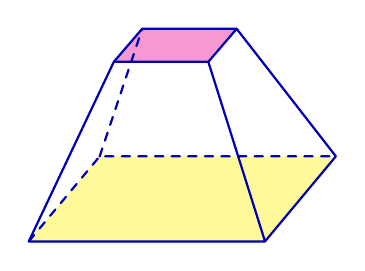
\begin{tikzpicture}[font=\footnotesize, line join=round, line cap=round, >=stealth, scale=0.6]
			
			\coordinate (B) at (0, 0);
			\coordinate (C) at (5, 0);
			\coordinate (D) at (6.5, 1.8);
			\coordinate (A) at (1.5, 1.8);
			
			\coordinate (B') at (1.8, 3.8);
			\coordinate (C') at (3.8, 3.8);
			\coordinate (D') at (4.4, 4.5);
			\coordinate (A') at (2.4, 4.5);
			
			
			\fill[yellow!40] (A) -- (B) -- (C) -- (D) -- cycle;
			\fill[magenta!40] (A') -- (B') -- (C') -- (D') -- cycle;
			
			
			\draw[dashed, thick, color=blue!70!black] (B) -- (A) -- (D)
			(A) -- (A');		
			\draw[thick, color=blue!70!black] (B) -- (C) -- (D)
			 (A') -- (B') -- (C') -- (D') -- cycle
			 (B) -- (B')
			 (C) -- (C')
			 (D) -- (D');
	\end{tikzpicture}}
		

		
	
	\shortans{40{,}5}
	\loigiai{
		\begin{center}
			\begin{tikzpicture}[font=\footnotesize, line join=round, line cap=round, >=stealth, scale=0.9]
			
				\coordinate (A) at (0,1.5);
				\coordinate (B) at (-2,0);
				\coordinate (C) at (3,0);
				\coordinate (D) at (5,1.5);
				
				\coordinate (O) at ($(A)!0.5!(C)$);
				
				\coordinate (O') at ($(O)+(0,3.5)$);
			
				\coordinate (E) at ($(O') + 0.4*(A) - 0.4*(O)$);
				\coordinate (F) at ($(O') + 0.4*(B) - 0.4*(O)$);
				\coordinate (G) at ($(O') + 0.4*(C) - 0.4*(O)$);
				\coordinate (H) at ($(O') + 0.4*(D) - 0.4*(O)$);
			
				\coordinate (I) at ($(O) + 0.4*(D) - 0.4*(O)$);
				\coordinate (J) at ($(O) + 0.4*(B) - 0.4*(O)$);
				
			
				\draw[dashed] (A)--(B) (A)--(D) (A)--(E) (B)--(D) (H)--(I) (F)--(J) (I)--(J);
				
				\draw (B)--(C)--(D) (B)--(F) (C)--(G) (D)--(H) (E)--(F)--(G)--(H)--cycle;
				
				
				\foreach \p/\pos in {A/left, B/below left, C/below right, D/right, E/above left, F/above left, G/above, H/above right, I/below, J/below}
				\fill (\p) circle (1.2pt) node[\pos] {$\p$};
			\end{tikzpicture}
		\end{center}
		
		\noindent Ký hiệu chân tháp là khối chóp cụt tứ giác đều có đáy lớn là $ABCD$ và đáy nhỏ là $EFGH$. Khi đó, thiết diện qua đường chéo là tứ giác $BDHF$ tạo thành một hình thang cân.\\
		Gọi $I, J$ lần lượt là hình chiếu vuông góc của $H, F$ lên mặt phẳng $(ABCD)$. \\
		Vì khối chóp cụt đều nên $I$, $J$ nằm trên đường chéo $BD$ và $IJ = FH$.\\
		Đường chéo đáy dưới $BD = \sqrt{AB^2+AD^2} = \sqrt{5^2+5^2} = 5\sqrt{2} \ (\text{m})$.\\
		Đường chéo đáy trên $FH = \sqrt{EF^2+EH^2} = \sqrt{2^2+2^2} = 2\sqrt{2} \ (\text{m})$.\\
		Ta có: 
		\[ BJ = DI = \dfrac{BD - IJ}{2} = \dfrac{5\sqrt{2} - 2\sqrt{2}}{2} = \dfrac{3\sqrt{2}}{2} \ (\text{m}). \]
		Xét tam giác $HID$ vuông tại $I$, chiều cao của khối chóp cụt là:
		\[ h = HI = \sqrt{HD^2 - ID^2} = \sqrt{3^2 - \left(\dfrac{3\sqrt{2}}{2}\right)^2} = \sqrt{9 - \dfrac{18}{4}} = \dfrac{3\sqrt{2}}{2} \ (\text{m}). \]
		Diện tích đáy dưới $S = 5^2 = 25 \ (\text{m}^2)$.\\
		Diện tích đáy trên $S' = 2^2 = 4 \ (\text{m}^2)$.\\
		Thể tích khối bê tông (khối chóp cụt) là
		\allowdisplaybreaks
		\begin{eqnarray*}
			V &=& \dfrac{h}{3}\left(S + S' + \sqrt{S \cdot S'}\right) \\
			&=& \dfrac{\frac{3\sqrt{2}}{2}}{3}\left(25 + 4 + \sqrt{25 \cdot 4}\right) \\
			&=& \dfrac{\sqrt{2}}{2} \cdot 39 = \dfrac{39\sqrt{2}}{2} \ (\text{m}^3).
		\end{eqnarray*}
		Số tiền mua bê tông tươi là
		\[ T = V \cdot 1\,470\,000 = \dfrac{39\sqrt{2}}{2} \cdot 1\,470\,000 \approx 40\,538\,431{,}77 \text{ (đồng)}. \]
		Vậy số tiền cần dùng xấp xỉ $40{,}5$ triệu đồng.
	}
\end{ex}

\begin{ex}%[2D1C3-6]%[TheHung, Dự án DeTHPT 2025 - 2026]
\immini{Chú kiến bị lạc tổ, chú đang loay hoay để tìm tổ. Chú đi theo suy đoán và đặt hệ trục tọa độ $Oxy$ thì đường đi của chú có quỹ đạo là một phần đường cong đồ thị hàm số có công thức $y = f(x) = a(x-b)^2$ (với $a,b$ là các số thực dương). Hàm số $y = f(x)$ có tính chất.
	Với số thực $k$ gọi hàm số $g(k) = \max\limits_{[k; k+2]} f(x) - \min\limits_{[k; k+2]} f(x)$. Hàm số $g(k)$ thỏa mãn
	$$\heva{& g(3) = a \\ & g(2) + g(6) = 32.}$$
	 }{\begin{tikzpicture}[>=stealth, scale=0.65, font=\footnotesize]
		\draw[->] (-1,0) -- (8.5,0) node[below] {$x$};
		\draw[->] (0,-1) -- (0,5) node[left] {$y$};
		\fill (0,0) circle (1.5pt) node[below left] {$O$};
		\draw[->, thick] (0,0) -- (1,0) node[below] {$\vec{i}$};
		\draw[->, thick] (0,0) -- (0,1) node[left] {$\vec{j}$};
		
		% Vẽ điểm A minh họa
		\draw[dashed] (7,0) node[below] {$7$} -- (7,4);
		\fill[red] (7,4) circle (2pt) node[above, text=black] {$A$};
\end{tikzpicture}}
	Biết tổ của chú nằm ngay tại gốc tọa độ $O$.	
Thời điểm $9$ giờ sáng chú đang ở vị trí $A$ (hình vẽ bên). Khoảng cách giữa chú kiến và tổ của mình là bao nhiêu? (kết quả làm tròn đến hàng phần chục).
		

	\shortans{19{,}3}
	\loigiai{
		Ta có hàm số $f(x) = a(x-b)^2$ với $a > 0$ là một parabol có đỉnh tại $x=b$, bề lõm hướng lên trên.\\
		Từ giả thiết $g(3) = a$, ta có
		\[ g(3) = \max_{[3;5]} f(x) - \min_{[3;5]} f(x) = a \left[ \max_{[3;5]} (x-b)^2 - \min_{[3;5]} (x-b)^2 \right] = a \]
		Vì $a > 0$, chia cả hai vế cho $a$, ta được $\max\limits_{[3;5]} (x-b)^2 - \min\limits_{[3;5]} (x-b)^2 = 1$. \quad $(*)$
		
		Xét sự biến thiên của hàm số $y=(x-b)^2$ trên đoạn $[3; 5]$, vị trí của đỉnh $x=b$ sẽ quyết định giá trị lớn nhất và nhỏ nhất. Ta xét 3 trường hợp:
		\begin{itemize}
			\item \textbf{Trường hợp 1: $b \le 3$.} Khi đó đỉnh nằm bên trái đoạn đang xét nên hàm số đồng biến trên $[3; 5]$.
			\[ (*) \Leftrightarrow (5-b)^2 - (3-b)^2 = 1 \Leftrightarrow 25 - 10b - 9 + 6b = 1 \Leftrightarrow 4b = 15 \Leftrightarrow b = \dfrac{15}{4} \text{ (loại vì $b \le 3$)}. \]
			\item \textbf{Trường hợp 2: $b \ge 5$.} Khi đó đỉnh nằm bên phải đoạn đang xét nên hàm số nghịch biến trên $[3; 5]$.
			\[ (*) \Leftrightarrow (3-b)^2 - (5-b)^2 = 1 \Leftrightarrow 9 - 6b - 25 + 10b = 1 \Leftrightarrow 4b = 17 \Leftrightarrow b = \dfrac{17}{4} \text{ (loại vì $b \ge 5$)}. \]
			\item \textbf{Trường hợp 3: $3 < b < 5$.} Khi đó đỉnh nằm trong đoạn đang xét nên $\min\limits_{[3;5]} (x-b)^2 = 0$ (đạt tại $x=b$) và $\max\limits_{[3;5]} (x-b)^2 = \max\left\{ (3-b)^2; (5-b)^2 \right\}$.\\ Phương trình $(*)$ trở thành
			\allowdisplaybreaks
			\begin{align*}
				\max\left\{ (3-b)^2; (5-b)^2 \right\} - 0 = 1 \Leftrightarrow \hoac{& (3-b)^2 = 1 \\ & (5-b)^2 = 1} \Leftrightarrow \hoac{& b = 2 \quad \text{(loại)} \\ & b = 4 \quad \text{(nhận)} \\ & b = 6 \quad \text{(loại)} \\ & b = 4 \quad \text{(nhận)}.}
			\end{align*}
			Vậy $b = 4$.
		\end{itemize}
		
		Với $b=4$, ta có $f(x) = a(x-4)^2$ mà theo giả thiết $g(2) + g(6) = 32$.
		\begin{itemize}
			\item Xét trên đoạn $[2; 4]$, đỉnh $x=4$ nằm ở biên phải, hàm số nghịch biến
			\[ g(2) = a\left[ \max_{[2;4]} (x-4)^2 - \min_{[2;4]} (x-4)^2 \right] = a\left[ (2-4)^2 - (4-4)^2 \right] = 4a. \]
			\item Xét trên đoạn $[6; 8]$, đỉnh $x=4$ nằm ngoài biên trái, hàm số đồng biến
			\[ g(6) = a\left[ \max_{[6;8]} (x-4)^2 - \min_{[6;8]} (x-4)^2 \right] = a\left[ (8-4)^2 - (6-4)^2 \right] = a(16 - 4) = 12a. \]
		\end{itemize}
		Ta có phương trình: $4a + 12a = 32 \Leftrightarrow 16a = 32 \Leftrightarrow a = 2$ (thỏa mãn $a > 0$).
		
		Do đó, hàm số mô tả quỹ đạo của chú kiến là $f(x) = 2(x-4)^2$. \\
		Tại thời điểm 9h sáng, chú kiến đang ở vị trí $A$ có hoành độ $x=7$ (theo hình vẽ minh họa). \\
		Tung độ của điểm $A$ là $y_A = f(7) = 2(7-4)^2 = 18 \Rightarrow A(7; 18)$.\\
		Khoảng cách từ chú kiến đến tổ (gốc tọa độ $O$) chính là độ dài đoạn thẳng $OA$
		\[ OA = \sqrt{7^2 + 18^2} = \sqrt{373} \approx 19{,}3. \]
		Vậy khoảng cách xấp xỉ là $19{,}3$ (đơn vị độ dài).
	}
\end{ex}

\begin{ex}%[0D2V2-3]%[TheHung, Dự án DeTHPT 2025 - 2026]
	Có ba nhóm máy A, B, C dùng để sản xuất ra hai loại sản phẩm I và II. Để sản xuất một đơn vị sản phẩm mỗi loại phải lần lượt dùng các máy thuộc các nhóm khác nhau. Số máy trong một nhóm và số máy của từng nhóm cần thiết để sản xuất ra một đơn vị sản phẩm thuộc mỗi loại được cho trong bảng sau:
	\begin{center}
		\renewcommand{\arraystretch}{1.5}
		\begin{tabular}{|c|c|c|c|}
			\hline
			\multirow{2}{*}{Nhóm} & \multirow{2}{*}{Số máy trong mỗi nhóm} & \multicolumn{2}{c|}{Số máy trong từng nhóm để sản xuất $1$ đvsp} \\
			\cline{3-4}
			& & \makebox[3.5cm]{Loại $I$} & \makebox[3.5cm]{Loại $II$} \\
			\hline
			$A$ & $10$ & $2$ & $2$ \\
			\hline
			$B$ & $4$ & $0$ & $2$ \\
			\hline
			$C$ & $12$ & $2$ & $4$ \\
			\hline
		\end{tabular}
	\end{center}	
	Một đơn vị sản phẩm $I$ lãi ba nghìn đồng, một đơn vị sản phẩm loại II lãi năm nghìn đồng. Trong điều kiện sản xuất đó hãy tính số tiền lãi có thể đạt cao nhất? (tiền lãi có đơn vị nghìn đồng).
	\shortans{17}
	\loigiai{
		Gọi $x, y$ lần lượt là số đơn vị sản phẩm loại $I, II$ cần sản xuất ($x \ge 0, y \ge 0$).\\
		Dựa vào bảng số liệu và điều kiện giới hạn số máy của mỗi nhóm, ta có hệ bất phương trình:
		\[ \heva{& x \ge 0 \\ & y \ge 0 \\ & 2x + 2y \le 10 \\ & 2y \le 4 \\ & 2x + 4y \le 12} \Leftrightarrow \heva{& x \ge 0 \\ & y \ge 0 \\ & x + y \le 5 \\ & y \le 2 \\ & x + 2y \le 6} \]
		Gọi $L(x; y)$ là tổng số tiền lãi thu được (đơn vị: nghìn đồng), ta có
		\[ L(x; y) = 3x + 5y \]
		Biểu diễn miền nghiệm của hệ bất phương trình trên mặt phẳng tọa độ $Oxy$, ta được miền ngũ giác $OABCD$ (miền được tô màu xám như hình vẽ):
		
		\begin{center}
			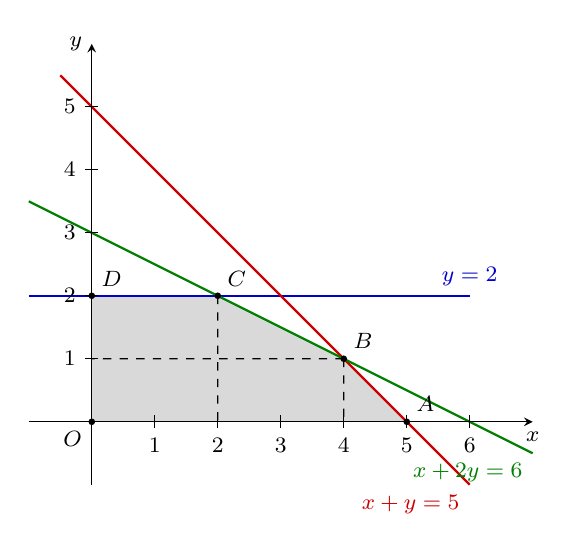
\begin{tikzpicture}[>=stealth, scale=0.8, font=\footnotesize]
				
				\fill[gray!30] (0,0) -- (5,0) -- (4,1) -- (2,2) -- (0,2) -- cycle;
				
				
				\draw[thick, blue!80!black] (-1,2) -- (6,2) node[above] {$y=2$};
				\draw[thick, red!80!black] (-0.5,5.5) -- (6,-1) node[below left] {$x+y=5$};
				\draw[thick, green!50!black] (-1,3.5) -- (7,-0.5) node[below left] {$x+2y=6$};
				
				
				\draw[->] (-1,0) -- (7,0) node[below] {$x$};
				\draw[->] (0,-1) -- (0,6) node[left] {$y$};
				\fill (0,0) circle (1.5pt) node[below left] {$O$};
				
				
				\foreach \x in {1,2,3,4,5,6}
				\draw (\x,0.1) -- (\x,-0.1) node[below] {$\x$};
				\foreach \y in {1,2,3,4,5}
				\draw (0.1,\y) -- (-0.1,\y) node[left] {$\y$};
				
				
				\coordinate (A) at (5,0);
				\coordinate (B) at (4,1);
				\coordinate (C) at (2,2);
				\coordinate (D) at (0,2);
				
				\fill (A) circle (1.5pt) node[above right] {$A$};
				\fill (B) circle (1.5pt) node[above right] {$B$};
				\fill (C) circle (1.5pt) node[above right] {$C$};
				\fill (D) circle (1.5pt) node[above right] {$D$};
				
				
				\draw[dashed] (B) -- (4,0)
				 (B) -- (0,1)
				 (C) -- (2,0);
			\end{tikzpicture}
		\end{center}
		
		Tọa độ các đỉnh của miền nghiệm là: $O(0;0), A(5;0), B(4;1), C(2;2), D(0;2)$.\\
		Thay tọa độ các đỉnh vào hàm mục tiêu $L(x; y) = 3x + 5y$, ta có:
		\begin{itemize}
			\item $L(O) = 3(0) + 5(0) = 0$
			\item $L(A) = 3(5) + 5(0) = 15$
			\item $L(B) = 3(4) + 5(1) = 17$
			\item $L(C) = 3(2) + 5(2) = 16$
			\item $L(D) = 3(0) + 5(2) = 10$
		\end{itemize}
		Giá trị lớn nhất của $L(x; y)$ là $17$, đạt được tại $x = 4, y = 1$.\\
		Vậy tiền lãi lớn nhất là $17$ nghìn đồng (khi sản xuất $4$ sản phẩm loại $I$ và $1$ sản phẩm loại $II$).
	}
\end{ex}

\Closesolutionfile{ans}

%\indapan{6}{ans/ans-15-26-2-NgheAn-LienTruong-L1-NLC}
%\indapan{4}{ans/ans-15-26-2-NgheAn-LienTruong-L1-DS}
%\indapan{6}{ans/ans-15-26-2-NgheAn-LienTruong-L1-KQ}
